\subsection{Parametric Function Fitting}
    For $A \in\mathbb{R}^{N \times M}$: \textit{Null Space} or \textit{Kernel} = subspace of all vectors $\mathbf{x}\in\mathbb{R}^N$ s.t. $A\mathbf{x}=0$. It is denoted by null($A$). \textit{Left Null Space} or \textit{Cokernel}: null($A^\top$). \textit{Column Space} or \textit{Range} or \textit{Image} of $A$ is the space spanned by the columns of A and is denoted by range($A$). \textit{Row Space} or \textit{Coimage} of $A$: range($A^\top$).
    
    We want to minimize error:
    \begin{equation*}
        \|\mathbf{e}\|_2=\sqrt{\sum_{i=1}^N e_i^2}=\sqrt{\sum_{i=1}^N (y_i-f(x_i))^2}
    \end{equation*}
    Choosing different norms yields different results.
    
    \textbf{N: \#Data Points \\M: \#Free Parameters/Functions}

\subsection{Linear Least Squares}
    Fit data $\left\{(x_i, y_i)\right\}_{i=1}^{N}$ with a function $f(x)$ which can be expressed as M linearly independent functions $\p_k(x)$,
    \begin{equation*}
        f(x;\textbf{\textit{w}}) = \sum_{k=1}^M w_k\p_k(x)
    \end{equation*}
    where $\textbf{\textit{w}}=(w_1, w_2, \dots, w_M)$ are the unknown weights.
    Functions can be nonlinear but \textbf{weights have to enter lineraly}.
    
    Goal: find \textbf{\textit{w}} s.t. error $E(\textbf{\textit{w}}) = \|\mathbf{e(\textbf{\textit{w}})}\|^2_2$ is minimised.
    \begin{equation*}
        \textbf{\textit{w}}^\star = \underset{\textbf{\textit{w}}}{\arg\min}\textrm{ } E(\textbf{\textit{w}})\Rightarrow \frac{d E(\textbf{\textit{w}})}{d \textbf{\textit{w}}} = 0
    \end{equation*}
    Matrix notation leads us to: $A\Vec{w}= \Vec{y}$
    \\$A\in\mathbb{R}^{N\times M}$, $\textbf{\textit{w}}\in\mathbb{R}^{M}$, $\textbf{\textit{y}}\in\mathbb{R}^{N}$
    \begin{equation*}
        \begin{bmatrix}
            \p_1(x_1) & \p_2(x_1) & \dots & \p_M(x_1)\\
            \p_1(x_2) & \p_2(x_2) & \dots & \p_M(x_2)\\
            \vdots & \ddots & & \vdots\\
            \vdots & & \ddots & \vdots\\
            \p_1(x_N) & \p_2(x_N) & \dots & \p_M(x_N)\\
        \end{bmatrix}
        \begin{bmatrix}
            w_1\\
            w_2\\
            \vdots\\
            w_M
        \end{bmatrix}
        = 
        \begin{bmatrix}
            y1\\
            y_2\\
            \vdots\\
            \vdots\\
            y_N
        \end{bmatrix}
    \end{equation*}
    \begin{itemize}
        \item M=N there exists unique solution $\textbf{\textit{w}} = A^{-1}\textbf{\textit{y}}$.
        \item M\textgreater N System is underdetermined and has infinitely many solutions
        \item M\textless N System is overdetermined. We can approximate a solution $A\textbf{\textit{w}}\approx \textbf{\textit{y}}$ with least squares requiring $E(\textbf{\textit{w}}) = \|\textbf{\textit{y}}-A\textbf{\textit{w}}\|_2^2$ be minimal.
    \end{itemize}
    \begin{equation*}
        \colorboxed{red}{
            \w^\star = (A^\top A)^{-1}A^\top\y
        }
    \end{equation*}
    
    \subsubsection{Solution for Linear Functions}
        Consider set of data $\{x_i, y_i\}_{i = 1}^N$ which we want to fit to $y = w_1 + w_2 x$
        \begin{equation*}
        \begin{bmatrix}
            1 & x_1\\
            1 & x_2\\
            \vdots & \vdots\\
            1 & x_N\\
        \end{bmatrix}
        \begin{bmatrix}
            w_1\\
            w_2\\
        \end{bmatrix}
        = 
        \begin{bmatrix}
            y1\\
            y_2\\
            \vdots\\
            y_N
        \end{bmatrix}
    \end{equation*}
    % \begin{equation*}
    %     \begin{bmatrix}
    %         N & \sum_{i=1}^N x_i\\
    %         \sum_{i=1}^N x_i & \sum_{i=1}^N x_i^2
    %     \end{bmatrix}
    %     \begin{bmatrix}
    %         w_1\\
    %         w_2\\
    %     \end{bmatrix}
    %     =
    %      \begin{bmatrix}
    %         \sum_{i=1}^N y_i\\
    %         \sum_{i=1}^N x_iy_i
    %     \end{bmatrix}
    % \end{equation*}
    \begin{equation*}
        w_1^\star = \frac{\sum_{i=1}^N x_i^2\sum_{i=1}^N y_i-\sum_{i=1}^N x_i\sum_{i=1}^N x_iy_i}{N\sum_{i=1}^N x_i^2-\left(\sum_{i=1}^N x_i\right)^2}
    \end{equation*}
    \begin{equation*}
        w_2^\star = \frac{N\sum_{i=1}^N x_iy_i-\sum_{i=1}^N x_i\sum_{i=1}^N y_i}{N\sum_{i=1}^N x_i^2-\left(\sum_{i=1}^N x_i\right)^2}
    \end{equation*}

    \subsubsection{Orthonormal Case}
        Let $\mathbf{a}_i$ be the columns of $A \in\mathbb{R}^{N\times M}$. Columns are orthogonal iff \begin{equation*}
            \mathbf{a}_i \cdot \mathbf{a}_j = \delta_{ij} \quad 1 \leq i,j \leq M
        \end{equation*}
        An \textit{orthogonal Matrix} has the following properties:
        \begin{equation*}
            A^\top = A^{-1}; \qquad \|A\mathbf{u}\| = \|\mathbf{u}\|
        \end{equation*}
        LSQ simplifies to:
        \begin{equation*}
            \textbf{\textit{w}}^\star = A^\top\textbf{\textit{y}}
        \end{equation*}
        % \TODO{example?}
        
    \subsection{Geometric Interpretation}
        The columns of A span a M-dimensionl space. The least squares method finds the solution $\w^\star$ s.t. $A\w^\star$ is the projection of $\y$ on the column space of $A$.
        We observe that the residual $\mathbf{e} = \mathbf{y}-A\w^\star$ is perpendicular to  range($A$) and has minimal 2-norm ($\|e\|=\|\y-A\w\|$ is minimal for $\w = \w^\star$)
        \begin{center}
            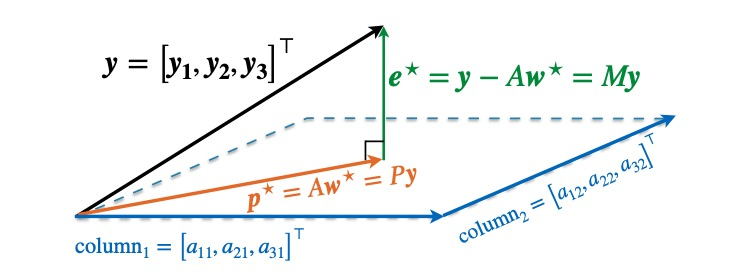
\includegraphics[width = 0.7\linewidth]{images/01/geometric_interpretation.jpg}\\
            Geometric interpretation for $N=3$ and $M = 2$
        \end{center}
        
        $\mathbf{e}^\star\in$ left nullspace $A$
        
        $A\w = \y$ has a solution iff $\y\in$ range $A$ $\Rightarrow \mathbf{e} = 0$
        \subsubsection{Projection Matrix P}
            closest point to $\y$ is $\Vec{p} = A\w^\star = P\Vec{y}$
            \begin{equation*}
                \colorboxed{red}{
                    P = A(A^\top A)^{-1}A^\top
                }
            \end{equation*}
            P is called a \textit{projection matrix} and has the following properties:
            \begin{equation*}
                P = P^\top \textrm{ (symmetric)}; \quad P^2 = P \textrm{ (idemptotent)}
            \end{equation*}
            
            We can write the error as $\Vec{e} = \y - A\w^\star =\y -P\y = M\y$
            \begin{equation*}
                M = \mathbb{I} - A(A^\top A)^{-1}A^\top
            \end{equation*}
            where $M$ is also a projection matrix, projecting onto null($A^\top$) (space orthogonal to the column space of $A$), whereas P projects onto range($A$)
            \begin{equation*}
                P + M = \mathbb{I}; \quad PM=0; \quad PA=A; \quad MA=0
            \end{equation*}
        
